\section{Empirical relevance}
\begin{frame}{Empirical relevance: definition}
    The \alert{empirical relevance} $r_i(t)$ of node $i$ at time $t$ is defined as:

    \[
        r_i(t) = \frac{n_i(t)}{n_i^{PA}(t)}
    \]

    \begin{itemize}
        \item $n_i(t) = \frac{\Delta k_i^{in}(t, \Delta t)}{L(t, \Delta t)}$: ratio between number of incoming links received by node $i$ in the time window $[t, t+\Delta t]$ and the total number of links created within the same time window
        \item $n_i^{PA}(t) = \frac{k_i^{in}(t)}{\sum_j k_j^{in}(t)}$: expected value of $n_i(t)$ according to preferential attachment alone
    \end{itemize}

    $r_i(t) > 1$ \alert{$(< 1)$}: node $i$ at time $t$ outperforms \alert{(underperforms)} in the competition for incoming links with respect to its preferencial attachment weight.
\end{frame}

\section{The Extended Fitness Model}

\begin{frame}{The Extended Fitness Model}
    \begin{itemize}
        \item \textbf{PageRank's under-performance in time-dependent networks is a general feature.}
        \item We can validate this using a model more compatible with the idea that \emph{a node is important if it's pointed by other important nodes.}
    \end{itemize}
    \begin{center}
        \alert{Extended Fitness Model} (EFM)
    \end{center}
    \begin{itemize}
        \item \textbf{High-fitness nodes are more sensitive to fitness} than low-fitness nodes, when choosing their outgoing links.
        \item High-fitness nodes are then more likely to be pointed by other high-fitness nodes than low-fitness nodes.
        \item EFM is \alert{more favorable} to PageRank than RM.
    \end{itemize}
\end{frame}

\begin{frame}{EFM:\@ sensitivity to fitness}
    Probability $\Pi_{i;j}^{in}(t)$ that a link created by node $j$ at time $t$ ends in node $i$:
    \[
        \Pi_{i;j}^{in}(t) \sim (k_i^{in}(t)+1)^{1-\eta_j} \, \eta_i^{\eta_j} \, f_R(t-\tau_i)
    \]
    \begin{itemize}
        \item Fitness $\eta \in [0, 1]$ to prevent negative exponents
        \item $\Pi^{in}$ depends on the fitness of the target \emph{and of the source} nodes (difference with RM).
        \item $k_i^{in}(t)$: indegree of node $i$ at time $t$.
    \end{itemize}
\end{frame}

\begin{frame}{PageRank vs.\ indegree: correlation with fitness in EFM}
    \begin{figure}
        \begin{columns}

        \column{0.6\textwidth}
            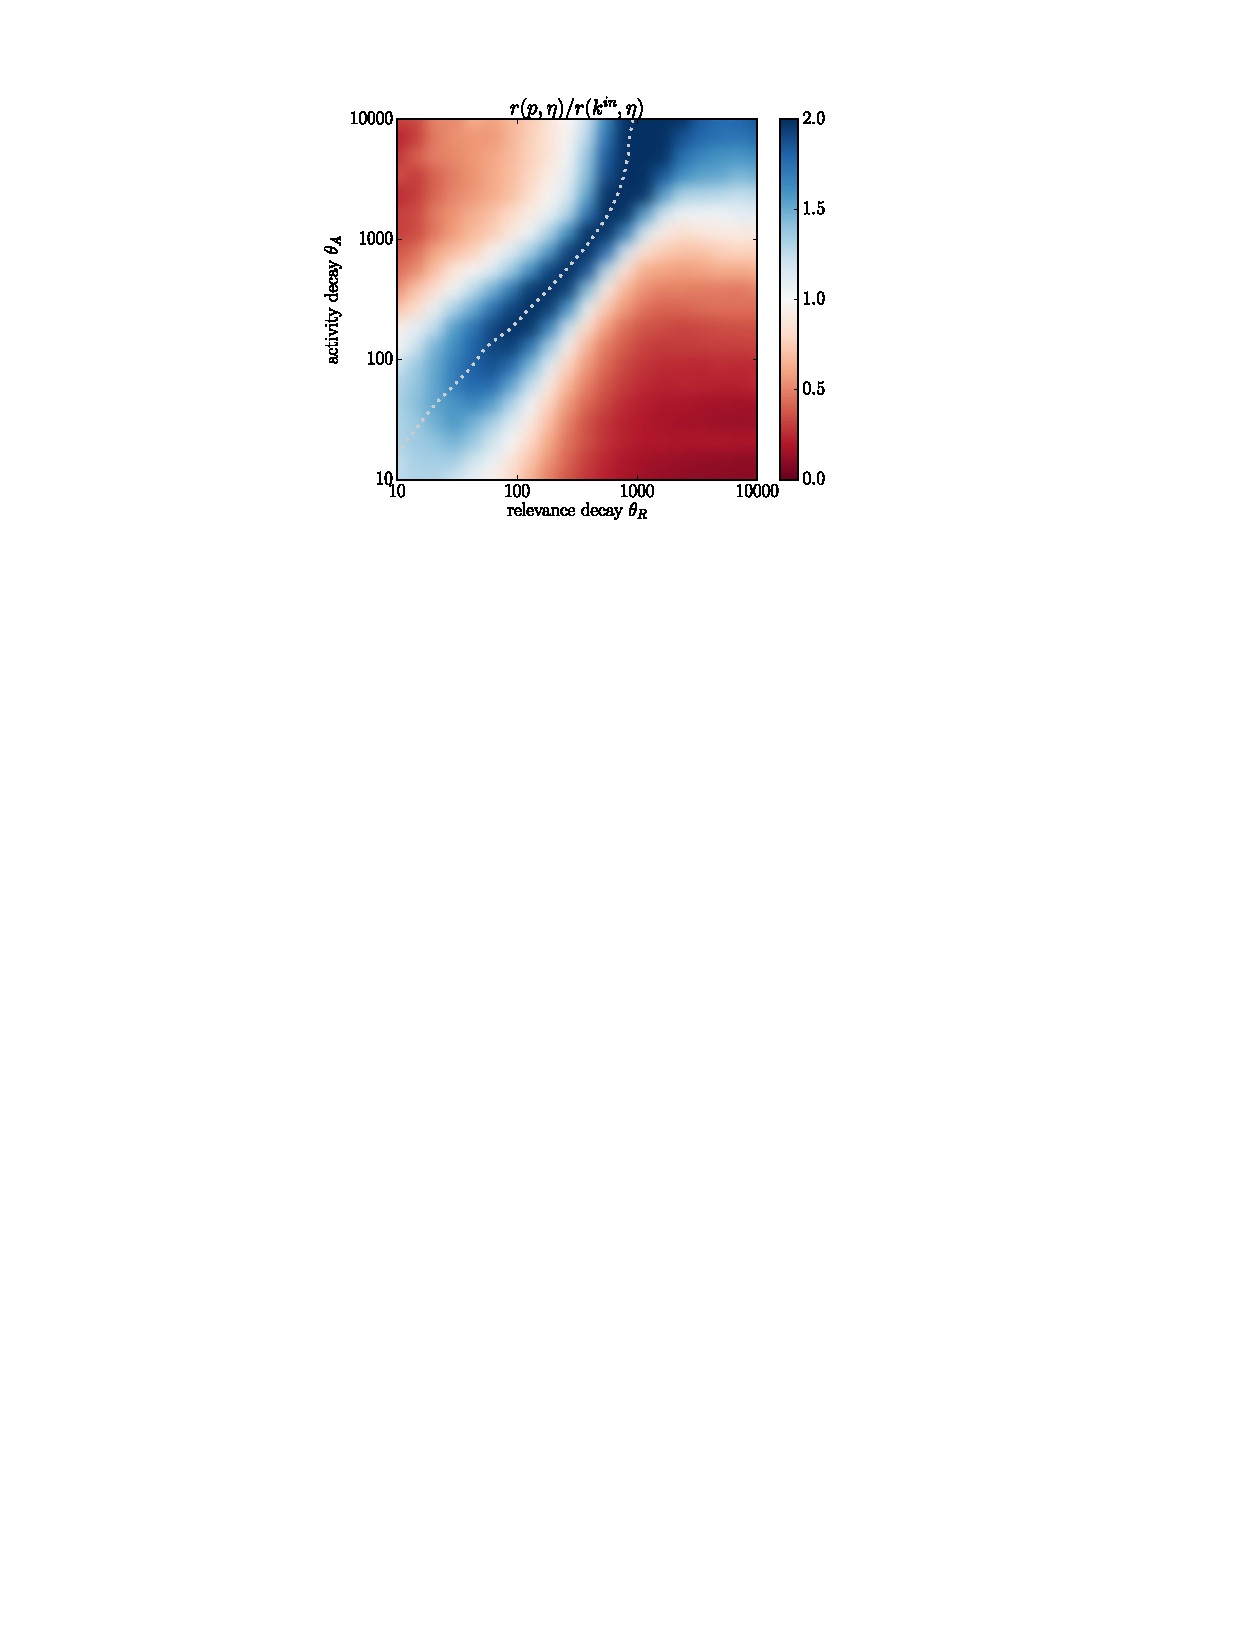
\includegraphics[width=1.0\textwidth]{figures/PageRankEFM_heatmap}

        \column{0.4\textwidth}
            \begin{footnotesize}
            \begin{itemize}
                \item $\rho(A) = 2A^{-3}, \; A \in [1, \infty]$
                \item $H$ nodes: high fitness; $\eta \in [10^{-5}, 1]$
                \item $(N-H)$ nodes: low fitness; $\eta \in [0, 10^{-5}]$
                \item $N=10000$, $H=250$
            \end{itemize}
            \end{footnotesize}
        \end{columns}
        \caption{Comparison of performance of PageRank and indegree (EFM data).}
    \end{figure}
\end{frame}
